\section{胶片与成像管道}\label{sec:胶片与成像管道}
相机中胶片或传感器类型对入射光转换为图像中颜色的方式具有戏剧性影响。
在pbrt中,类\refvar{Film}{}在模拟相机中对传感设备建模。
在为每条相机光线求得辐亮度后,\refvar{Film}{}的实现
决定了样本对胶片平面上的相机光线起始点周围像素的贡献并更新其图像表示。
当主渲染循环退出时,\refvar{Film}{}将最终图像写入文件。

对于真实相机模型,\refsub{相机测量方程}介绍了测量方程,
它描述了相机中的传感器怎样度量一段时间内到达传感器区域上的能量大小。
对于更简单的相机模型,我们可将传感器视作度量某段时间内一小片区域上的平均辐亮度。
选择采用哪种度量的影响被封装在\refvar[GenerateRayDifferential]{Camera::GenerateRayDifferential}{()}为
光线返回的权重中。因此,\refvar{Film}{}的实现
可在不考虑这些变化的情况下处理,只需用这些权重缩放提供的辐亮度。

本节介绍了单个\refvar{Film}{}实现,它将像素重建方程应用于计算最终像素值。
对于基于物理的渲染器,通常最好是把结果图像存于浮点图像格式。
这样做在如何使用输出方面比起用8位无符号整数值的传统图像格式提供了更多的灵活性;
浮点格式避免了将图像量化为8位时造成的大量信息损失。

为了在现代显示设备上显示这样的图像,有必要将这些浮点像素值映射为离散值。
例如,计算机监视器通常希望每个像素的颜色由一个RGB颜色三元组描述,
而不是用任意的光谱功率分布。因此通用基函数系数描述的光谱在能显示之前必须转化为RGB表示。
一个相关问题是,比起许多真实世界场景中出现的范围,
显示器具有小得多的可显示辐亮度值范围。因此,像素值必须
以让最终显示的图像看起来尽可能接近其在无限制的理想显示设备上的样子的方式映射到可显示的范围。
这些问题是通过研究\keyindex{色调映射}{tone mapping}{}来解决的;
“扩展阅读”一节有关于该话题的更多信息。

\subsection{胶片类}\label{sub:胶片类}
\refvar{Film}{}定义在文件\href{https://github.com/mmp/pbrt-v3/blob/master/src/core/film.h}{\ttfamily core/film.h}
和\href{https://github.com/mmp/pbrt-v3/blob/master/src/core/film.cpp}{\ttfamily core/film.cpp}中。
\begin{lstlisting}
`\initcode{Film Declarations}{=}\initnext{FilmDeclarations}`
class `\initvar{Film}{}` {
public:
    `\refcode{Film Public Methods}{}`
    `\refcode{Film Public Data}{}`
private:
    `\refcode{Film Private Data}{}`
    `\refcode{Film Private Methods}{}`
};
\end{lstlisting}
\begin{lstlisting}
`\initcode{Film Public Methods}{=}`
`\refvar{Film}{}`(const `\refvar{Point2i}{}` &resolution, const `\refvar{Bounds2f}{}` &cropWindow,
    std::unique_ptr<`\refvar{Filter}{}`> filter,
    `\refvar{Float}{}` diagonal, const std::string &filename, `\refvar{Float}{}` scale);
`\refvar{Bounds2i}{}` `\refvar{GetSampleBounds}{}`() const;
`\refvar{Bounds2f}{}` `\refvar{GetPhysicalExtent}{}`() const;
std::unique_ptr<`\refvar{FilmTile}{}`> `\refvar{GetFilmTile}{}`(const `\refvar{Bounds2i}{}` &sampleBounds);
void `\refvar{MergeFilmTile}{}`(std::unique_ptr<`\refvar{FilmTile}{}`> tile);
void `\refvar{SetImage}{}`(const `\refvar{Spectrum}{}` *img) const;
void `\refvar{AddSplat}{}`(const `\refvar{Point2f}{}` &p, const `\refvar{Spectrum}{}` &v);
void `\refvar[Film::WriteImage]{WriteImage}{}`(`\refvar{Float}{}` splatScale = 1);
void `\refvar[Film::Clear]{Clear}{}`();
\end{lstlisting}

许多值传给了构造函数:图像以像素为单位的整个分辨率;
可能指定了要渲染的图像子集的裁剪窗口;
胶片物理区域的对角线长度,它在构造函数中单位是毫米,但这里转换为了米;
一个滤波函数;输出图像的文件名以及控制图像像素值如何存于文件的参数。
\begin{lstlisting}
`\initcode{Film Method Definitions}{=}\initnext{FilmMethodDefinitions}`
`\refvar{Film}{}`::`\refvar{Film}{}`(const `\refvar{Point2i}{}` &resolution, const `\refvar{Bounds2f}{}` &cropWindow,
        std::unique_ptr<`\refvar{Filter}{}`> filt, `\refvar{Float}{}` diagonal,
        const std::string &filename, `\refvar{Float}{}` scale)
    : `\refvar{fullResolution}{}`(resolution), `\refvar{diagonal}{}`(diagonal * .001),
    `\refvar{filter}{}`(std::move(filt)), `\refvar{filename}{}`(filename), `\refvar{scale}{}`(scale) {
    `\refcode{Compute film image bounds}{}`
    `\refcode{Allocate film image storage}{}`
    `\refcode{Precompute filter weight table}{}`
}
\end{lstlisting}

\begin{lstlisting}
`\initcode{Film Public Data}{=}\initnext{FilmPublicData}`
const `\refvar{Point2i}{}` `\initvar{fullResolution}{}`;
const `\refvar{Float}{}` `\initvar{diagonal}{}`;
std::unique_ptr<`\refvar{Filter}{}`> `\initvar{filter}{}`;
const std::string `\initvar{filename}{}`;
\end{lstlisting}

裁剪窗口于整体图像分辨率结合起来给出了实际需要存储和写出的像素边界。
裁剪窗口对于调试或将大图像分解为可在不同电脑上渲染的小块然后重新组装很有用。
裁剪窗口是在NDC空间中指定的,每个坐标范围是0到1(\reffig{7.47})。
\begin{figure}[htbp]
    \centering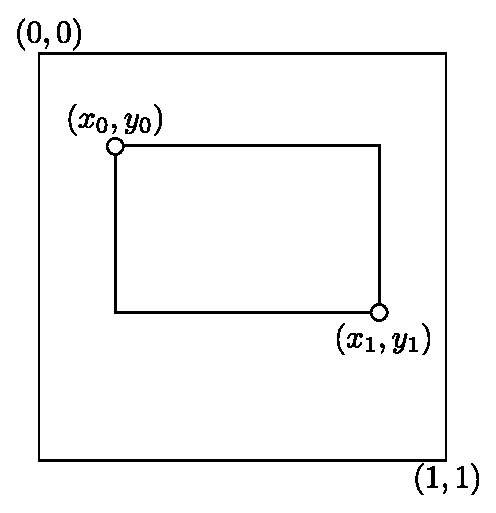
\includegraphics[width=0.5\linewidth]{chap07/Cropwindow.eps}
    \caption{图像裁剪窗口指定要渲染的图像子集。
    它在NDC空间中给出,坐标范围为从$(0,0)$到$(1,1)$.
    类\refvar{Film}{}仅为裁剪窗口内的区域分配空间存储像素值。}
    \label{fig:7.47}
\end{figure}

\refvar[croppedPixelBounds]{Film::croppedPixelBounds}{}保存了
裁剪窗口从左上角到右下角的像素边界。小数像素坐标被舍入;
这保证了如果图像按邻接的裁剪窗口分块渲染,则最终像素只在一个子图像内出现。
\begin{lstlisting}
`\initcode{Compute film image bounds}{=}`
`\refvar{croppedPixelBounds}{}` =
    `\refvar{Bounds2i}{}`(`\refvar{Point2i}{}`(std::ceil(`\refvar{fullResolution}{}`.x * cropWindow.pMin.x),
                     std::ceil(`\refvar{fullResolution}{}`.y * cropWindow.pMin.y)),
             `\refvar{Point2i}{}`(std::ceil(`\refvar{fullResolution}{}`.x * cropWindow.pMax.x),
                     std::ceil(`\refvar{fullResolution}{}`.y * cropWindow.pMax.y)));
\end{lstlisting}
\begin{lstlisting}
`\refcode{Film Public Data}{+=}\lastcode{FilmPublicData}`
`\refvar{Bounds2i}{}` `\initvar{croppedPixelBounds}{}`;
\end{lstlisting}

有了(可能被裁的)图像像素分辨率后,构造函数
为每个像素分配一个\refvar{Pixel}{}结构体数组。
光谱像素贡献值的运行加权和用XYZ颜色(\refsub{XYZ颜色})表示
并保存于成员变量\refvar[Pixel:xyz]{xyz}{}中。
\refvar[Pixel:filterWeightSum]{filterWeightSum}{}
持有表示样本对像素的贡献的滤波权重值之和。
\refvar[Pixel:splatXYZ]{splatXYZ}{}持有样本背板
\sidenote{译者注:此短语翻译不确定,原文sample splats。欢迎读者提供帮助。}(不加权)的和。
成员\refvar[Pixel:pad]{pad}{}是没用的;
它唯一的目的是保证结构体\refvar{Pixel}{}是32字节大小,而不是28
(这里假设\refvar{Float}{}是4字节;否则它保证是64字节结构体)。
该填充保证了\refvar{Pixel}{}不会跨越缓存行,
这样当获取\refvar{Pixel}{}时引发的缓存缺失不超过一次
(只要数组的首个\refvar{Pixel}{}是在缓存行开头分配的)。
\begin{lstlisting}
`\initcode{Film Private Data}{=}\initnext{FilmPrivateData}`
struct `\initvar{Pixel}{}` {
    `\refvar{Float}{}` `\initvar[Pixel:xyz]{xyz}{}`[3] = { 0, 0, 0 };
    `\refvar{Float}{}` `\initvar[Pixel:filterWeightSum]{filterWeightSum}{}` = 0;
    `\refvar{AtomicFloat}{}` `\initvar[Pixel:splatXYZ]{splatXYZ}{}`[3];
    `\refvar{Float}{}` `\initvar[Pixel:pad]{pad}{}`;
};
std::unique_ptr<`\refvar{Pixel}{}`[]> `\initvar[Pixel::pixels]{pixels}{}`;
\end{lstlisting}
\begin{lstlisting}
`\initcode{Allocate film image storage}{=}`
`\refvar[Pixel::pixels]{pixels}{}` = std::unique_ptr<`\refvar{Pixel}{}`[]>(new `\refvar{Pixel}{}`[`\refvar{croppedPixelBounds}{}`.Area()]);
\end{lstlisting}
用XYZ颜色存储像素值的两个自然选择是用\refvar{Spectrum}{}值或存储RGB值。
这里即使是在进行全光谱渲染时也不值得保存完整的\refvar{Spectrum}{}值。
因为写入到输出文件的最终颜色不包括\refvar{Spectrum}{}样本全集,
所以这里转换为三刺激值和先保存\refvar{Spectrum}{}再转换
为图像输出上的三刺激值相比并不代表损失了信息。
该情况下如果\refvar{Spectrum}{}有大量样本,
则不保存完整的\refvar{Spectrum}{}值能节约大量内存
(如果pbrt支持把\refvar{SampledSpectrum}{}值保存到文件,则需要重新考虑该设计选择)。

我们已选择用XYZ颜色而不是RGB以强调XYZ是独立于显示器的颜色表示,
而RGB需要假定显示器响应曲线的特定集合(\refsub{RGB颜色})。
(然而最后我们还是不得不转换为RGB,因为很少有图像文件格式保存XYZ颜色。)

有了典型的滤波器设置,每个图像样本都可能对最终图像中的16个或更多像素作出贡献。
特别是对于在光线相交测试和着色计算上花费相对较少时间的简单场景,
花在为每个样本更新图像上的时间会很多。
因此,\refvar{Film}{}预先计算滤波值的表使得
我们可以免去对方法\refvar{Filter::Evaluate}{()}的虚函数调用开销
以及推算滤波器的开销,而可以为滤波使用来自表中的值。
实践中不在每个样本的精确位置上推算滤波而引入的误差并不明显。

这里的实现做了合理假设即滤波器定义满足$f(x,y)=f(|x|,|y|)$,
所以表格只需要为滤波偏移量正象限存储值。
该假设对于pbrt中目前所有可用的\refvar{Filter}{}都成立且在实践中对大多数滤波器成立。
这让表的大小变为四分之一并改进了内存访问的一致性,
使缓存性能更好\footnote{这里该实现可进一步利用目前pbrt中所有滤波器都是可分离的事实,
只分配两个1D表。然而,为了允许更容易地添加不同滤波函数,我们这里没有假定可分离性。}。
\begin{lstlisting}
`\initcode{Precompute filter weight table}{=}`
int offset = 0;
for (int y = 0; y < `\refvar{filterTableWidth}{}`; ++y) {
    for (int x = 0; x < `\refvar{filterTableWidth}{}`; ++x, ++offset) {
        `\refvar{Point2f}{}` p;
        p.x = (x + 0.5f) * `\refvar{filter}{}`->`\refvar[Filter::radius]{radius}{}`.x / `\refvar{filterTableWidth}{}`;
        p.y = (y + 0.5f) * `\refvar{filter}{}`->`\refvar[Filter::radius]{radius}{}`.y / `\refvar{filterTableWidth}{}`;
        `\refvar{filterTable}{}`[offset] = filter->`\refvar[Filter::Evaluate]{Evaluate}{}`(p);
    }
}
\end{lstlisting}
\begin{lstlisting}
`\refcode{Film Private Data}{+=}\lastnext{FilmPrivateData}`
static constexpr int `\initvar{filterTableWidth}{}` = 16;
`\refvar{Float}{}` `\initvar{filterTable}{}`[`\refvar{filterTableWidth}{}` * `\refvar{filterTableWidth}{}`];
\end{lstlisting}

\begin{lstlisting}
`\refcode{Film Method Definitions}{+=}\lastnext{FilmMethodDefinitions}`
`\refvar{Bounds2i}{}` `\refvar{Film}{}`::`\initvar{GetSampleBounds}{()}` const {
    `\refvar{Bounds2f}{}` floatBounds(
        `\refvar{Floor}{}`(`\refvar{Point2f}{}`(`\refvar{croppedPixelBounds}{}`.pMin) + `\refvar{Vector2f}{}`(0.5f, 0.5f) -
              `\refvar{filter}{}`->`\refvar[Filter::radius]{radius}{}`),
        `\refvar{Ceil}{}`( `\refvar{Point2f}{}`(`\refvar{croppedPixelBounds}{}`.pMax) - `\refvar{Vector2f}{}`(0.5f, 0.5f) +
              `\refvar{filter}{}`->`\refvar[Filter::radius]{radius}{}`));
    return (`\refvar{Bounds2i}{}`)floatBounds;
}
\end{lstlisting}
\begin{lstlisting}
`\refcode{Film Method Definitions}{+=}\lastnext{FilmMethodDefinitions}`
`\refvar{Bounds2f}{}` `\refvar{Film}{}`::`\initvar{GetPhysicalExtent}{}`() const {
    `\refvar{Float}{}` aspect = (`\refvar{Float}{}`)`\refvar{fullResolution}{}`.y / (`\refvar{Float}{}`)`\refvar{fullResolution}{}`.x;
    `\refvar{Float}{}` x = std::sqrt(`\refvar{diagonal}{}` * `\refvar{diagonal}{}` / (1 + aspect * aspect));
    `\refvar{Float}{}` y = aspect * x;
    return `\refvar{Bounds2f}{}`(`\refvar{Point2f}{}`(-x / 2, -y / 2), `\refvar{Point2f}{}`(x / 2, y / 2));
}
\end{lstlisting}
\subsection{为胶片提供像素值}\label{sub:为胶片提供像素值}
\begin{lstlisting}
`\refcode{Film Method Definitions}{+=}\lastnext{FilmMethodDefinitions}`
std::unique_ptr<`\refvar{FilmTile}{}`> `\refvar{Film}{}`::`\initvar{GetFilmTile}{}`(
        const `\refvar{Bounds2i}{}` &sampleBounds) {
    `\refcode{Bound image pixels that samples in sampleBounds contribute to}{}`
    return std::unique_ptr<`\refvar{FilmTile}{}`>(new FilmTile(tilePixelBounds,
        filter->radius, filterTable, filterTableWidth));
}
\end{lstlisting}

\begin{lstlisting}
`\refcode{Film Declarations}{+=}\lastcode{FilmDeclarations}`
class `\initvar{FilmTile}{}` {
public:
    `\refcode{FilmTile Public Methods}{}`
private:
    `\refcode{FilmTile Private Data}{}`
};
\end{lstlisting}

\begin{lstlisting}
`\initcode{FilmTile Public Methods}{=}\initnext{FilmTilePublicMethods}`
`\refvar{FilmTile}{}`(const `\refvar{Bounds2i}{}` &pixelBounds, const `\refvar{Vector2f}{}` &filterRadius,
    const `\refvar{Float}{}` *filterTable, int filterTableSize)
    : `\refvar{pixelBounds}{}`(pixelBounds), `\refvar{filterRadius}{}`(filterRadius),
    `\refvar{invFilterRadius}{}`(1 / filterRadius.x, 1 / filterRadius.y),
    `\refvar{filterTable}{}`(filterTable), `\refvar{filterTableSize}{}`(filterTableSize) {
    `\refvar[FilmTile::pixels]{pixels}{}` = std::vector<`\refvar{FilmTilePixel}{}`>(std::max(0, pixelBounds.Area()));
}
\end{lstlisting}

\begin{lstlisting}
`\initcode{FilmTile Private Data}{=}`
const `\refvar{Bounds2i}{}` `\initvar{pixelBounds}{}`;
const `\refvar{Vector2f}{}` `\initvar{filterRadius}{}`, `\initvar{invFilterRadius}{}`;
const `\refvar{Float}{}` *`\initvar{filterTable}{}`;
const int `\initvar{filterTableSize}{}`;
std::vector<`\refvar{FilmTilePixel}{}`> `\initvar[FilmTile::pixels]{pixels}{}`;
\end{lstlisting}

\begin{lstlisting}
`\refcode{FilmTile Public Methods}{+=}\lastnext{FilmTilePublicMethods}`
void `\initvar{AddSample}{}`(const `\refvar{Point2f}{}` &pFilm, const `\refvar{Spectrum}{}` &L,
    `\refvar{Float}{}` sampleWeight = 1.) {
    `\refcode{Compute sample's raster bounds}{}`
    `\refcode{Loop over filter support and add sample to pixel arrays}{}`
}
\end{lstlisting}

\begin{lstlisting}
`\initcode{Compute sample's raster bounds}{=}`
`\refvar{Point2f}{}` pFilmDiscrete = pFilm - `\refvar{Vector2f}{}`(0.5f, 0.5f);
`\refvar{Point2i}{}` p0 = (`\refvar{Point2i}{}`)`\refvar{Ceil}{}`(pFilmDiscrete - filterRadius);
`\refvar{Point2i}{}` p1 = (`\refvar{Point2i}{}`)`\refvar{Floor}{}`(pFilmDiscrete + filterRadius) + `\refvar{Point2i}{}`(1, 1);
p0 = `\refvar[Point3::Max]{Max}{}`(p0, pixelBounds.pMin);
p1 = `\refvar[Point3::Min]{Min}{}`(p1, pixelBounds.pMax);
\end{lstlisting}

\begin{lstlisting}
`\refcode{Film Method Definitions}{+=}\lastnext{FilmMethodDefinitions}`
void `\refvar{Film}{}`::`\initvar{MergeFilmTile}{}`(std::unique_ptr<`\refvar{FilmTile}{}`> tile) {
    std::lock_guard<std::mutex> lock(`\refvar{mutex}{}`);
    for (`\refvar{Point2i}{}` pixel : tile->`\refvar{GetPixelBounds}{}`()) {
        `\refcode{Merge pixel into Film::pixels}{}`
    }
}
\end{lstlisting}
\begin{lstlisting}
`\refcode{Film Private Data}{+=}\lastnext{FilmPrivateData}`
std::mutex `\initvar{mutex}{}`;
\end{lstlisting}
\begin{lstlisting}
`\refcode{FilmTile Public Methods}{+=}\lastcode{FilmTilePublicMethods}`
`\refvar{Bounds2i}{}` `\initvar{GetPixelBounds}{}`() const { return `\refvar{pixelBounds}{}`; }
\end{lstlisting}
\begin{lstlisting}
`\refcode{Film Private Data}{+=}\lastcode{FilmPrivateData}`
const `\refvar{Float}{}` `\initvar{scale}{}`;
\end{lstlisting}

\subsection{图像输出}\label{sub:图像输出}
\begin{lstlisting}
`\refcode{Film Method Definitions}{+=}\lastcode{FilmMethodDefinitions}`
void `\refvar{Film}{}`::`\initvar[Film::WriteImage]{WriteImage}{}`(`\refvar{Float}{}` splatScale) {
    `\refcode{Convert image to RGB and compute final pixel values}{}`
    `\refcode{Write RGB image}{}`
}
\end{lstlisting}